\begin{event}{LinBox Winter days 2019}{LinBoxWinterDays2019}{Richerenches (FR),
2018-12-04 to 2018-18-07}{UJF}{10}{4}{https://github.com/linbox-team/fflas-ffpack/wiki/LinBox-winter-days-in-Richerenches-(Dec.-18)}

\textbf{\ODK implication.} \ODK participants: A. Breust, J-G. Dumas, C. Pernet, H. Zhu.

\ODK provided the main funding source for the workshop (accommodation,
subsistence and some travel expenses), for about 3.5k\euro.

\textbf{Event summary.} The LinBox Winter Days 2018 took place in Richerenches
(France) from December 4th to 7th.
There were 10 participants from either Université Grenoble Alpes or Université of Montpellier. The focus of the meeting
was twofold: advancing core development of the libraries in the LinBox ecosystem, and welcoming and integrating new
developpers within the community. The main activities of the group during the meeting were:
\begin{itemize}
\item group brainstorming on new designs (e.g. refactorization of the dense matrix classes, of lifting containers, etc),
\item pair programming of the resulting new designs,
\item close interraction in bug correction and code review,
\item tutorial presentations for introducing new developpers to the librairies.
\end{itemize}

\textbf{Results and impact.} A large number of issues and bugs have been successfully processed. New design for the
lifting container classes and the dense matrix classes have been finalized and their implementation drafted. This effort
was then successfully pursued and merged into the libraries.


\begin{figure}[ht]
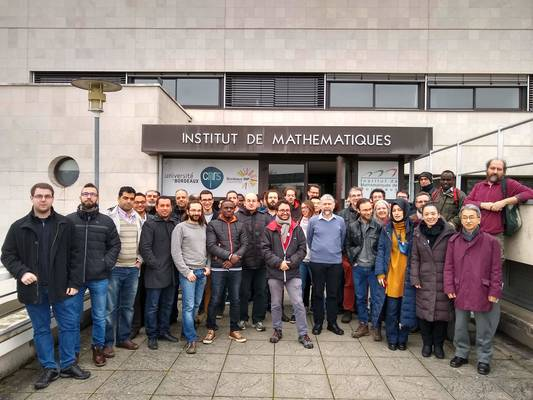
\includegraphics[scale=0.5]{pari2019.jpg}
\caption*{PARI/GP Atelier 2019 in Bordeaux}
\end{figure}

\end{event}
